\documentclass[a4paper]{article}
\newcommand{\sepspace}{\vspace*{1em}}	
%% Language and font encodings
\usepackage[english]{babel}
\usepackage[utf8x]{inputenc}
\usepackage[T1]{fontenc}
\usepackage{float}

%% Sets page size and margins
\usepackage[a4paper,top=3cm,bottom=2cm,left=3cm,right=3cm,marginparwidth=1.75cm]{geometry}

%% Useful packages
\usepackage{amsmath}
\usepackage{graphicx}

\title{ZND detonation of hydrogen and oxygen}
\author{Krzysztof Ufnal}

\begin{document}
\maketitle


% pierwsza sekcja
\section{Introduction}\label{sec:intro}
In this report one will find a study about ZND detonation using mixture of oxygen and hydrogen. There is a connection between detonation cell size and induction time, which will be calculated in this paper. This program calculates induction time which usually is considered to equal zero.  
\section{Mathematical model}\label{sec:model}
The ZND detonation model is a one-dimensional model for the process of detonation of an explosive. 
It was proposed during World War II independently by Y. B. Zel'dovich, John von Neumann, and Werner Döring, hence the name. 
This model admits finite-rate chemical reactions and thus the process of detonation consists of the following stages. 
First, an infinitely thin shock wave compresses the explosive to a high pressure called the von Neumann spike. 
At the von Neumann spike point the explosive still remains unreacted. 
The spike marks the onset of the zone of exothermic chemical reaction, which finishes at the Chapman-Jouguet state. 
After that, the detonation products expand backward. 
In the reference frame in which the shock is stationary, the flow following the shock is subsonic. 
Because of this, energy release behind the shock is able to be transported acoustically to the shock for its support. 
For a self-propagating detonation, the shock relaxes to a speed given by the Chapman–Jouguet condition, which induces the material at the end of the reaction zone to have a locally sonic speed in the reference frame in which the shock is stationary. 
In effect, all of the chemical energy is harnessed to propagate the shock wave forward.
However, in the 1960s, experiments revealed that gas-phase detonations were most often characterized by unsteady, three-dimensional structures, which can only in an averaged sense be predicted by one-dimensional steady theories. 
Indeed, such waves are quenched as their structure is destroyed. The Wood-Kirkwood detonation theory can correct for some of these limitations.
ZND code has been downloaded from Caltech website. 

\section{Results}\label{sec:results}

\begin{figure}[H]
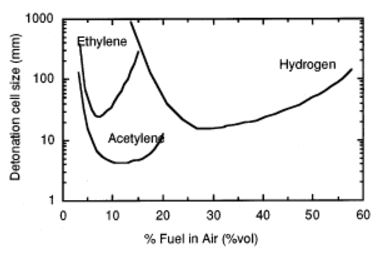
\includegraphics[width=1\textwidth]{cellsize.JPG}
\caption{\label{fig:cj}Experiments data}
\end{figure}

\begin{figure}[H]
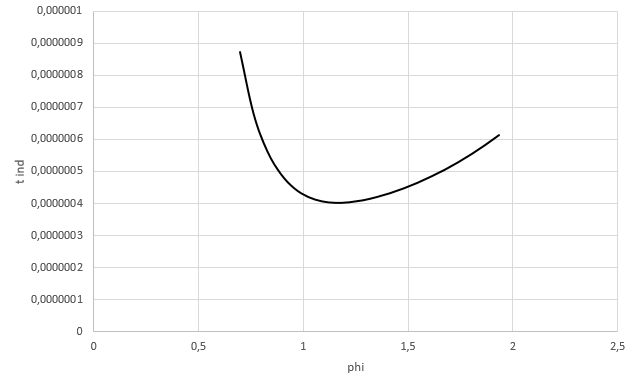
\includegraphics[width=1\textwidth]{ZND_KU.JPG}
\caption{\label{fig:p}Calculated ZND detonation}
\end{figure}

These two charts has similar properties, there is a relation which will be calculated below:

\begin{equation}
    a = t_ind/\lambda=7,77E-08/0,0121=6,65E-06
 \end{equation}   

\section{Summary}\label{sec:summary}
Program for calculating ZND detonation produced related to experiments results. Induction time happened to be measured in $seconds^-8$. Detonation of hydrogen with oxygen is extremely fast, this is why this mixture is called Knallgas (Scandinavian and German Knallgas: "bang-gas").


\section{References}\label{sec:refs}

 
[1] ZND program  \newline
$http://shepherd.caltech.edu/EDL/public/cantera/html/SD\_Toolbox/ZND$

[2] Properties of Hydrogen \newline
$http://www.cnbyxf.com/Doc/data.WebNoteBooks2010/07/20100728122525$

[3] Model description \newline
$https://en.wikipedia.org/wiki/ZND\_detonation\_model$


\end{document}
